\documentclass{article}

% if you need to pass options to natbib, use, e.g.:
%     \PassOptionsToPackage{numbers, compress}{natbib}
% before loading neurips_2021

% Silence warning about neurips package
\usepackage{silence}
\WarningFilter{latex}{You have requested package}

% ready for submission
%\usepackage{../neurips/neurips_2021}

% to compile a preprint version, e.g., for submission to arXiv, add add the
% [preprint] option:
\usepackage[preprint]{../neurips/neurips_2021}

% to compile a camera-ready version, add the [final] option, e.g.:
%\usepackage[final]{../neurips/neurips_2021}

% to avoid loading the natbib package, add option nonatbib:
%    \usepackage[nonatbib]{neurips_2021}

\usepackage[utf8]{inputenc} % allow utf-8 input
\usepackage[T1]{fontenc}    % use 8-bit T1 fonts
\usepackage{hyperref}       % hyperlinks
\usepackage{url}            % simple URL typesetting
\usepackage{booktabs}       % professional-quality tables
\usepackage{amsfonts}       % blackboard math symbols
\usepackage{nicefrac}       % compact symbols for 1/2, etc.
\usepackage{microtype}      % microtypography
\usepackage{xcolor}         % colors
\usepackage{amsmath}
\usepackage{graphicx}
\usepackage[inline]{enumitem}

% Set bibliography style for natbib (called out by the nips style file)
\bibliographystyle{abbrvnat}

% argmax and argmin operators
\DeclareMathOperator*{\argmax}{argmax}
\DeclareMathOperator*{\argmin}{argmin}

\title{ECE 239AS Reinforcement Learning\\
       Project Milestone Report}

% The \author macro works with any number of authors. There are two commands
% used to separate the names and addresses of multiple authors: \And and \AND.
%
% Using \And between authors leaves it to LaTeX to determine where to break the
% lines. Using \AND forces a line break at that point. So, if LaTeX puts 3 of 4
% authors names on the first line, and the last on the second line, try using
% \AND instead of \And before the third author name.

\author{%
    Ryan Chau \\
    \texttt{chau\_ryan@yahoo.com}\\
    \And
    My-Quan Hong \\
    \texttt{myquan@yahoo.com} \\
    % examples of more authors
    \And
    Nathan Kang \\
    \texttt{nkang@gseis.ucla.edu} \\
    \And
    Christopher Munoz \\
    \texttt{cmunozcortes@ucla.edu} \\
}

\begin{document}

\maketitle

\section{Introduction}
The objective of this project is to describe Double Deep Q Networks (DQN), an
algorithm first proposed in \citet{van2016deep} to reduce overoptimistic
action-value estimates in Deep Q Networks (\cite{mnih2015human}). A discussion
of another improvement on Deep Q Networks, Dueling DQN (\cite{wang2016dueling}),
will also be included for a more comprehensive survey.  Finally, a comparison of
the performance of all three algorithms on four Atari games will be presented.

Although Q-learning is one of the most popular reinforcement learning
algorithms, it is known to overestimate action values because of the included
maximization step. This issue extends to Deep Q-learning networks (DQN), which
combines Q-learning with a flexible deep neural network to approximate the
action-value function. Double Q-learning, which was proposed to alleviate the
overestimation issue in Q-learning, was subsequently shown to be effective in
solving the weaknesses of DQN and producing state-of-the-art results in the
Atari environment.

%------------------------------------------------------------------------------%
% TODO: Nathan & Ryan to include discussion on Dueling DQN
%------------------------------------------------------------------------------%

\section{Preliminary Results}
To conduct an evaluation of the performance of the algorhtms we used an
implementation based on the Tensorpack framework (\cite{wu2016tensorpack}).
Tensorpack is an interface built on TensorFlow v1 that is focused on training
speed. Its low overhead and support for training with a GPU provided us with a
way to train the models from scratch in Google Colab Pro instances, within a
reasonable amount of time (roughly 24 hours for each Atari game).

Each model was trained for 6.225 million training steps (250 epochs) on the
following games from the Atari Learning Environment (ALE)
(\cite{bellemare2013arcade}): \texttt{Breakout-v0}, \texttt{RoadRunner-v0},
\texttt{Boxing-v0}, and \texttt{VideoPinball-v0}.

Figure \ref{fig:training} shows the scores achieved by each trained model for
each of the four Atari games.

\begin{figure}[ht]
    \centering
    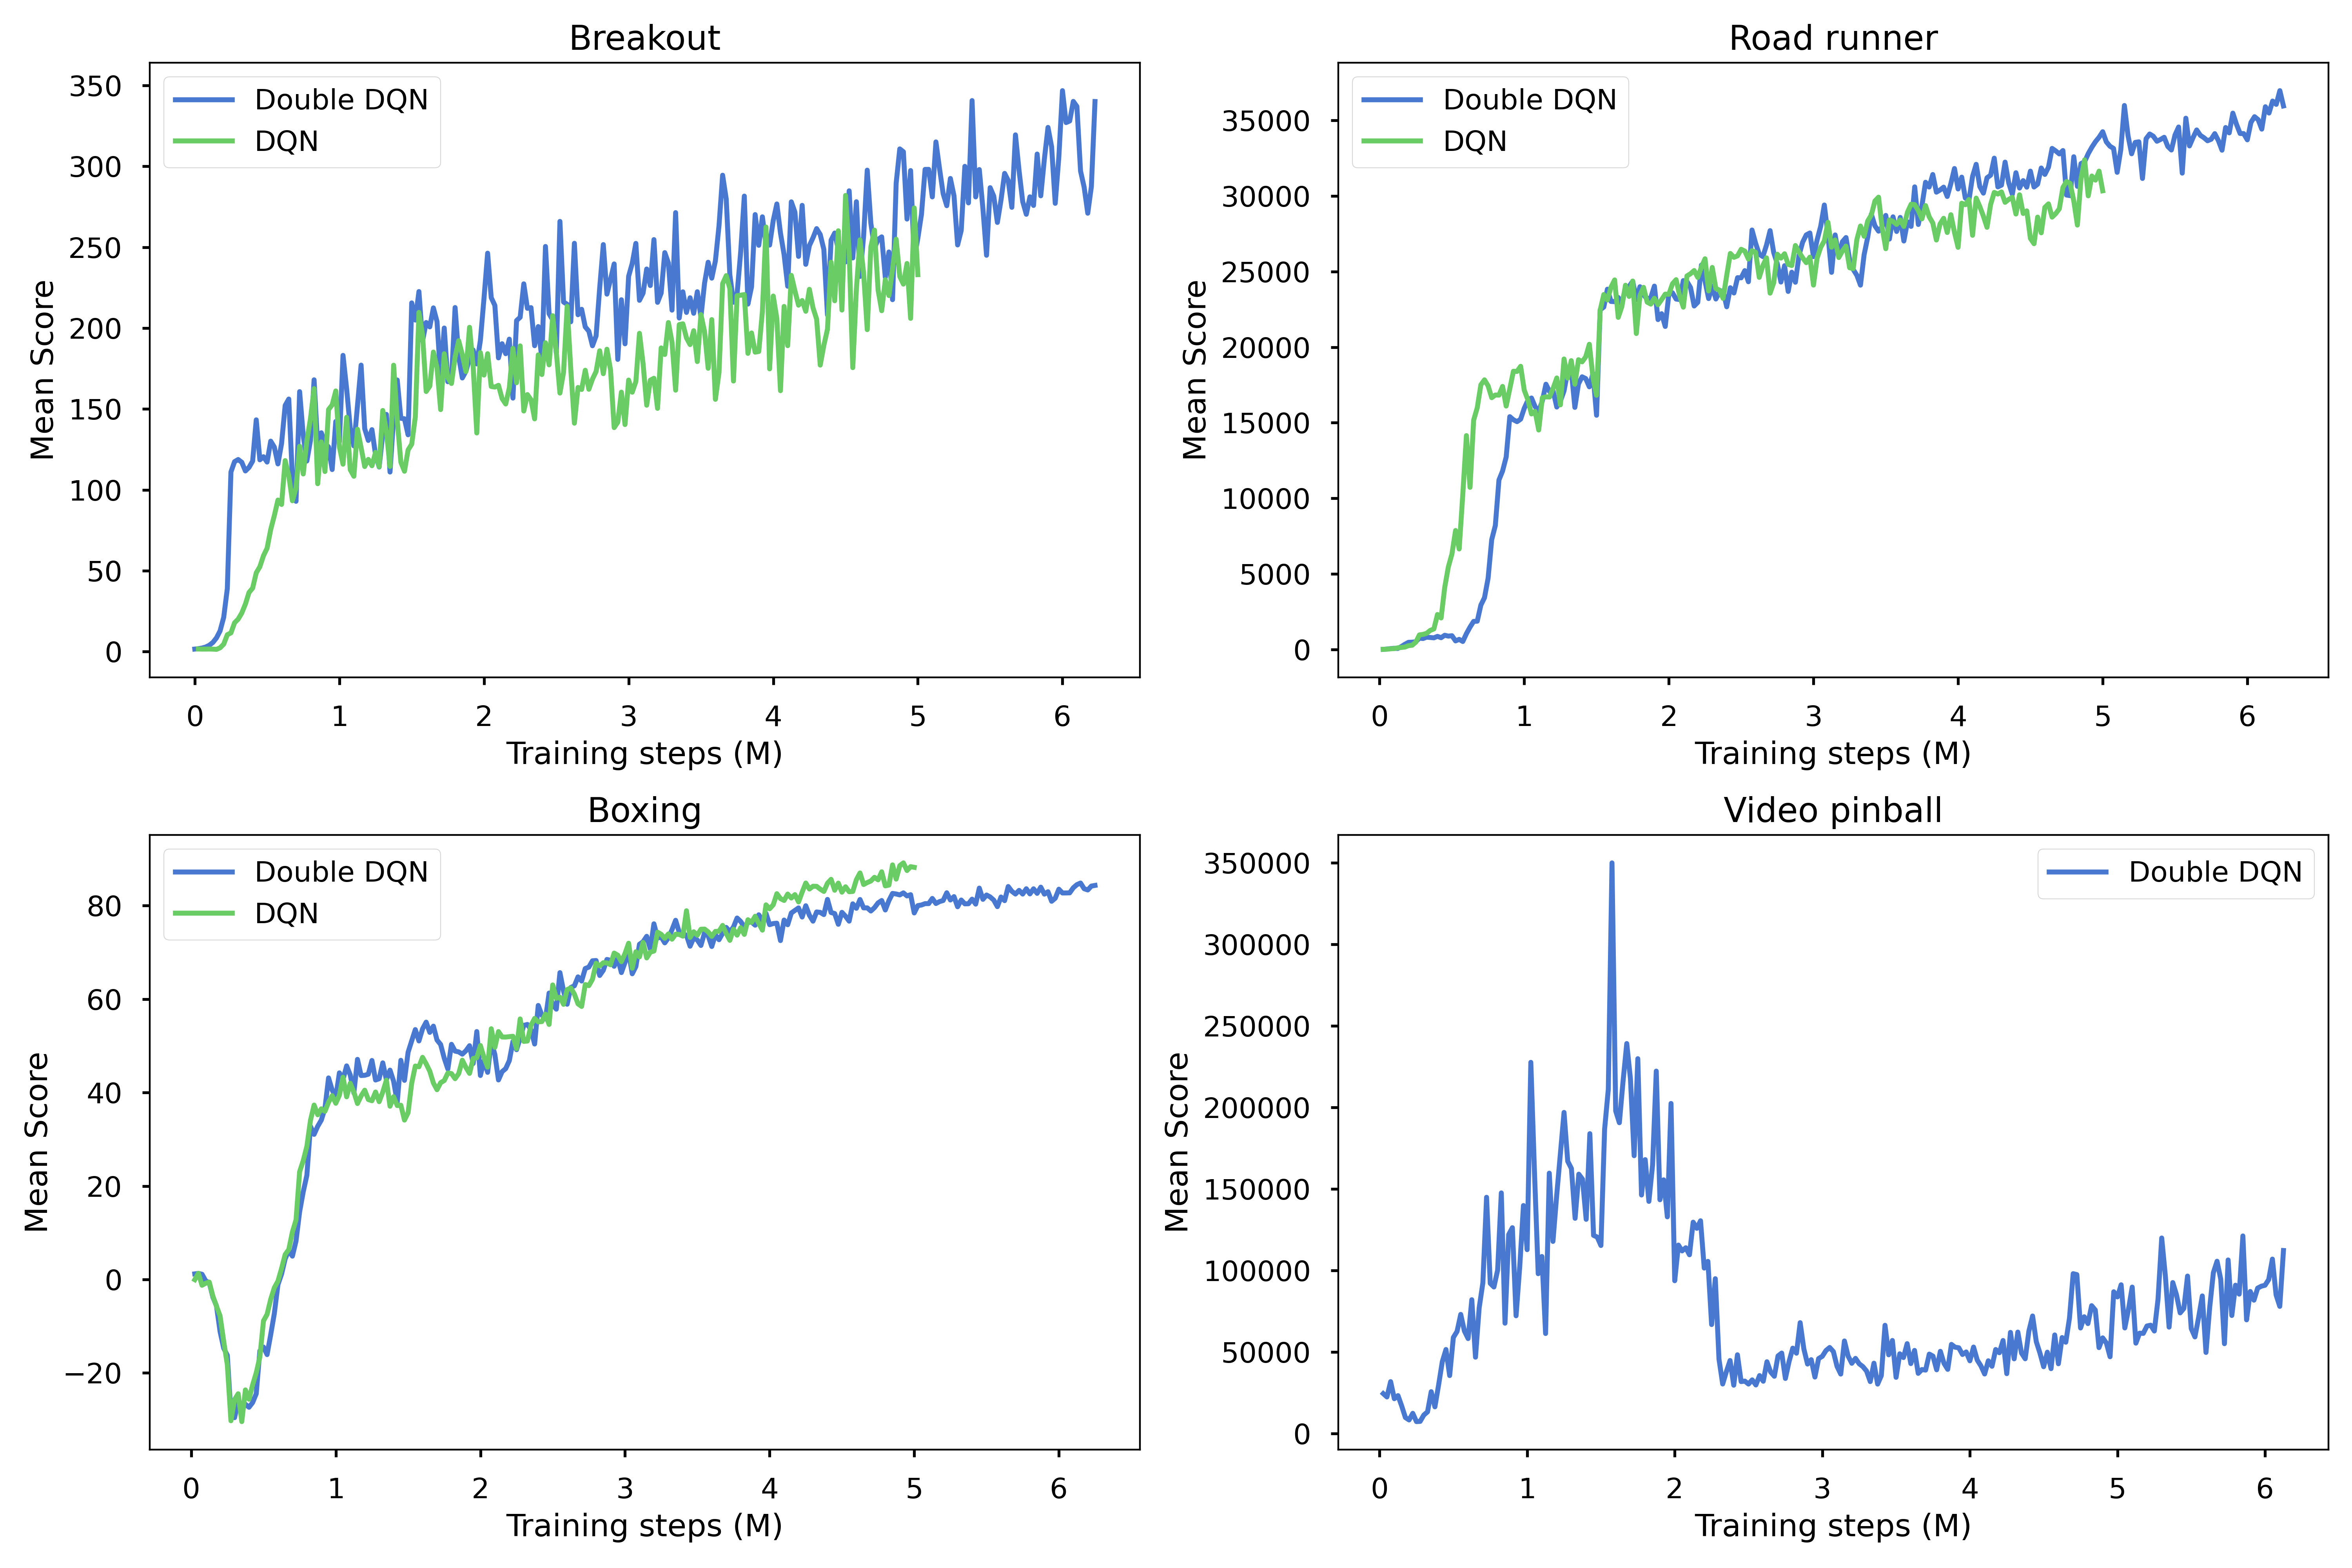
\includegraphics[width=\linewidth]{double_dqn-mean_scores.png}
    \caption{Mean score over training steps for selected games from the Atari
    Learning Environment (ALE).}
    \label{fig:training}
\end{figure}

The mean scores achieved by DQN and Double DQN were comparable on Road Runner
and Boxing. However, Double DQN performed better than DQN on Breakout and Video
Pinball, demonstrating the negative effects of DQN's overestimations.

% Import bibliography from ref.bib
\bibliography{ref}

\end{document}
